% Licensed to the Apache Software Foundation (ASF) under one or more
% contributor license agreements. See the NOTICE file distributed with
% this work for additional information regarding copyright ownership.
% The ASF licenses this file to You under the Apache License, Version 2.0
% (the ``License''); you may not use this file except in compliance with
% the License. You may obtain a copy of the License at
%
% http://www.apache.org/licenses/LICENSE-2.0
%
% Unless required by applicable law or agreed to in writing, software
% distributed under the License is distributed on an ``AS IS'' BASIS,
% WITHOUT WARRANTIES OR CONDITIONS OF ANY KIND, either express or implied.
% See the License for the specific language governing permissions and
% limitations under the License.

\subsubsection{Configuring a Documentum Authority Connection}

The following options apply specifically to a Documentum authority
connector.  A Documentum authority connector manages document security
to a repository in conjunction with the Documentum server (or
``docbroker'') specified in the GTS appliance configuration.  Each
Documentum authority connector connects to only one Documentum
repository (or ``docbase''). If the docbroker used by the GTS
appliance has access to more than one docbase, you will need to create
an authority connector for each repository you wish to crawl.

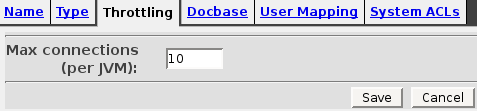
\includegraphics[width=300pt]{Docu-edit-authority-tab3}

\begin{itemize}

\item \textbf{Max Connections (per JVM):} The maximum number of
connections per JVM is important for two reasons.
\ifCombinedConnectorGuide \label{max-auth}\fi First, the number of
connections may impact the licensing on your document server,
depending on the repository. If you have a finite number of Documentum
connections available, they will be split between the authority
connector, which authorizes user access to documents, and the
repository connector, which actually downloads the documents to the
appliance. A default Documentum installation will have 100 connections
available; your Documentum installation may have more or less. It may
be advisable to lower the number of connections available to the
authority connector from the default value of 10. Ask your Documentum
administrator how many connections are available for use on your
Documentum system.

Second, the number of connections may impact the resources available
on the appliance. If the connector framework is slowing down your
appliance, lowering this number should help.

\end{itemize}

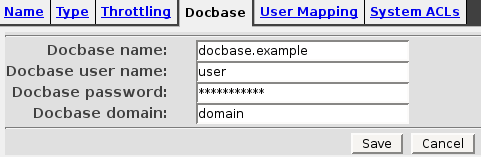
\includegraphics[width=300pt]{Docu-edit-authority-tab4}

\begin{itemize}

\item \textbf{Docbase name:} The host name of the Documentum
repository (or ``docbase'') with which you wish to connect.

\item \textbf{Docbase user name:} The user name that the GTS appliance
will use to connect to the docbase for this authority connection.
Typically, your Documentum administrator will create this account
specifically for use by the appliance. The account used by the GTS
appliance must have sufficient authority to retrieve user and group
ACLs.

\item \textbf{Docbase password:} The password corresponding to the
username given to the GTS.

\item \textbf{Docbase domain:} The domain that the docbase is part of,
typically an Active Directory domain. This is an optional argument.

\end{itemize}

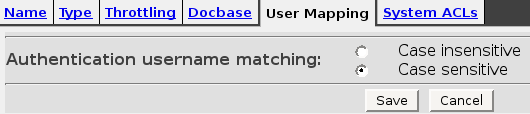
\includegraphics[width=300pt]{Docu-edit-authority-tab5}

\begin{itemize}

\item \textbf{Authentication username matching:} This option sets case
sensitivity for usernames.

\end{itemize}


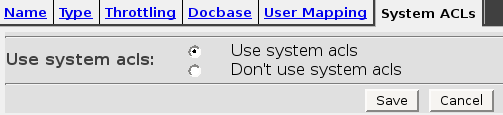
\includegraphics[width=300pt]{Docu-edit-authority-tab6}

\begin{itemize}

\item \textbf{Use system acls:} This option sets whether the GTS
appliance will use system-defined ACLs. The Documentum system
automatically generates an ACL for every folder in a docbase. Often,
ACLs of this kind are not assigned to users or groups. If your
Documentum security configuration does not use these automatically
generated ACLs, you should disable this option. The GTS appliance will
then only consider user-defined ACLs when determining file
permissions, increasing performance.

\end{itemize}




After entering this information, you will be taken to the authority
connection status page for this authority:

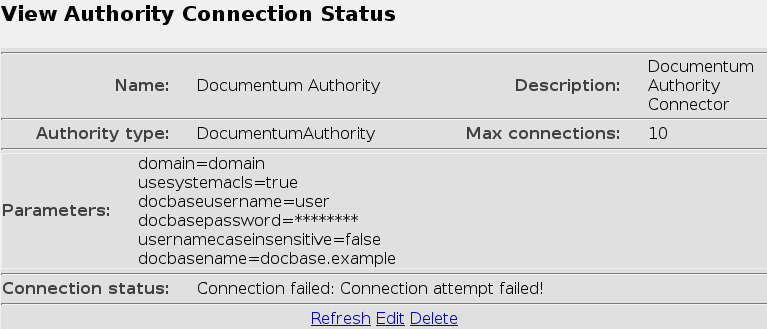
\includegraphics[width=300pt]{Docu-view-auth-conn-status}

In this example (which does not contain accurate information for any
Documentum server), the Connection Status is ``Connection failed.''
If you see this message, you most likely have incorrectly entered one
of the fields, and should click ``Edit'' to fix the data. If you have
entered everything as you intended, please inform your Documentum
administrator; you may not have been given the correct information.
